\begin{figure}[htbp]
\centering
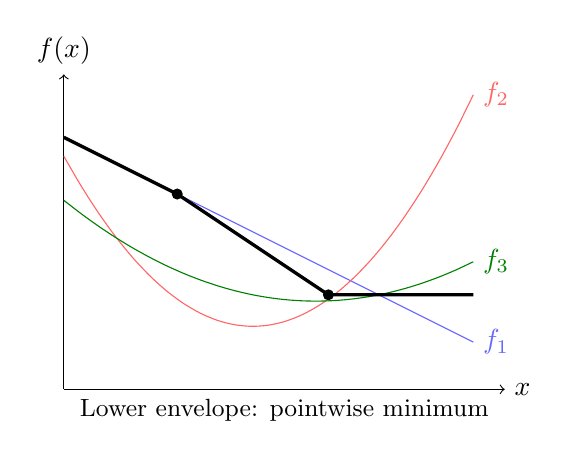
\begin{tikzpicture}[scale=0.8]
  \draw[->] (0,0)--(7,0) node[right] {$x$};
  \draw[->] (0,0)--(0,5) node[above] {$f(x)$};
  \draw[blue!60,domain=0:6.5,smooth] plot (\x,{4-0.5*\x}) node[right,blue!60] {$f_1$};
  \draw[red!60,domain=0:6.5,smooth] plot (\x,{1+0.3*(\x-3)^2}) node[right,red!60] {$f_2$};
  \draw[green!50!black,domain=0:6.5,smooth] plot (\x,{3-0.8*\x+0.1*\x*\x}) node[right,green!50!black] {$f_3$};
  \draw[very thick,black] (0,4) -- (1.8,3.1) -- (4.2,1.5) -- (6.5,1.5);
  \fill (1.8,3.1) circle (2.5pt);
  \fill (4.2,1.5) circle (2.5pt);
  \node[below,font=\small] at (3.5,0) {Lower envelope: pointwise minimum};
\end{tikzpicture}
\caption{Lower envelope of three functions: the thick black curve is the pointwise minimum $\min\{f_1, f_2, f_3\}$.}
\label{fig:lower_envelope}
\end{figure}
